\documentclass{scrartcl}
\usepackage{amsmath,amssymb,commath,graphicx}
\setkomafont{disposition}{\normalfont\bfseries}

\title{Numerical Analysis}
\subtitle{Homework C}
\author{Kenny Roffo}
\date{Due March 30}

\begin{document}

\maketitle

Fit a third order polynomial, $P_3(x)$, to $f(x)=x^5$ on $[-1,1]$ with least square error:\\

\textbf{a)}$P_3(x)=b_0+b_1x+b_2x^2+b_3x^3$ derive and then solve the normal equations.\\

\begin{align*}
E&=\int_{-1}^{1}(x^5-P_3(x))^2\dif{x}\\
&=\int_{-1}^{1}(x^5-b_0-b_1x-b_2x^2-b_3x^3)^2\dif{x}\\
&=\int_{-1}^{1}(x^{10}-b_0x^5-b_1x^6-b_2x^7-b_3x^8)+(-b_0x^5+{b_0}^2+b_0b_1x+b_0b_2x^2+b_0b_3x^3)\\
&\hspace{0.5 in}+(-b_1x^6+b_0b_1x+{b_1}^2x^2+b_1b_2x^3+b_1b_3x^4)+(-b_2x^7+b_0b_2x^2+b_1b_2x^3+{b_2}^2x^4+b_2b_3x^5)\\
&\hspace{0.5 in}+(-b_3x^8+b_0b_3x^3+b_1b_3x^4+b_2b_3x^5+{b_3}^2x^6)\dif{x}\\
&=\Bigg[\frac{x^{11}}{11}-\frac{b_0x^6}{6}-\frac{b_1x^7}{7}-\frac{b_2x^8}{8}-\frac{b_3x^9}{9}-\frac{b_0x^6}{6}+{b_0}^2x+\frac{b_0b_1x^2}{2}+\frac{b_0b_2x^3}{3}+\frac{b_0b_3x^4}{4}\\
&\hspace{0.5 in}-\frac{b_1x^7}{7}+\frac{b_0b_1x^2}{2}+\frac{{b_1}^2x^3}{3}+\frac{b_1b_2x^4}{4}+\frac{b_1b_3x^5}{5}-\frac{b_2x^8}{8}+\frac{b_0b_2x^3}{3}+\frac{b_1b_2x^4}{4}\\
&\hspace{0.5 in}+\frac{{b_2}^2x^5}{5}+\frac{b_2b_3x^6}{6}-\frac{b_3x^9}{9}+\frac{b_0b_3x^4}{4}+\frac{b_1b_3x^5}{5}+\frac{b_2b_3x^6}{6}+\frac{{b_3}^2x^7}{7}\Bigg]_{-1}^1\\
\end{align*}
\begin{align*}
&=\frac{1}{11}-\frac{b_0}{6}-\frac{b_1}{7}-\frac{b_2}{8}-\frac{b_3}{9}-\frac{b_0}{6}+{b_0}^2+\frac{b_0b_1}{2}+\frac{b_0b_2}{3}+\frac{b_0b_3}{4}\\
&\hspace{0.5 in}-\frac{b_1}{7}+\frac{b_0b_1}{2}+\frac{{b_1}^2}{3}+\frac{b_1b_2}{4}+\frac{b_1b_3}{5}-\frac{b_2}{8}+\frac{b_0b_2}{3}+\frac{b_1b_2}{4}\\
&\hspace{0.5 in}+\frac{{b_2}^2}{5}+\frac{b_2b_3}{6}-\frac{b_3}{9}+\frac{b_0b_3}{4}+\frac{b_1b_3}{5}+\frac{b_2b_3}{6}+\frac{{b_3}^2}{7}\\
&\hspace{0.5 in}+\frac{1}{11}+\frac{b_0}{6}-\frac{b_1}{7}+\frac{b_2}{8}-\frac{b_3}{9}+\frac{b_0}{6}+{b_0}^2-\frac{b_0b_1}{2}+\frac{b_0b_2}{3}-\frac{b_0b_3}{4}\\
&\hspace{0.5 in}-\frac{b_1}{7}-\frac{b_0b_1}{2}+\frac{{b_1}^2}{3}-\frac{b_1b_2}{4}+\frac{b_1b_3}{5}+\frac{b_2}{8}+\frac{b_0b_2}{3}-\frac{b_1b_2}{4}\\
&\hspace{0.5 in}+\frac{{b_2}^2}{5}-\frac{b_2b_3}{6}-\frac{b_3}{9}-\frac{b_0b_3}{4}+\frac{b_1b_3}{5}-\frac{b_2b_3}{6}+\frac{{b_3}^2}{7}\\
&=-\frac{4}{7}b_1-\frac{4}{9}b_3+2{b_0}^2+\frac{2}{3}{b_1}^2+\frac{2}{5}{b_2}^2+\frac{2}{7}{b_3}^2+\frac{4}{3}b_0b_2+\frac{4}{5}b_1b_3+\frac{2}{11}
\end{align*}
We now find the partial derivatives of $E$ with respect to each $b_i$ to get an inconsistent system of linear equations:
\begin{align*}
\dpd{E}{b_0}&=4b_0+\frac{4}{3}b_2\\
\dpd{E}{b_1}&=-\frac{4}{7}+\frac{4}{3}b_1+\frac{4}{5}b_3\\
\dpd{E}{b_2}&=\frac{4}{5}b_2+\frac{4}{3}b_0\\
\dpd{E}{b_3}&=-\frac{4}{9}+\frac{4}{7}b_3+\frac{4}{5}b_1
\end{align*}
Now, setting these equal to zero we have:
\begin{align*}
3b_0+b_2&=0\\
35b_1+21b_3&=15\\
5b_0+3b_2&=0\\
63b_1+45b_3&=35
\end{align*}
We are now able to represent this system of equations with matrices:
\begin{displaymath}
\begin{bmatrix}
3 & 0 & 1 & 0\\
0 & 35 & 0 & 21\\
5 & 0 & 3 & 0\\
0 & 63 & 0 & 45 
\end{bmatrix}
\begin{bmatrix}
b_0\\
b_1\\
b_2\\
b_3
\end{bmatrix}
= \begin{bmatrix}
0\\
15\\
0\\
35
\end{bmatrix}
\end{displaymath}
Now we multiply both sides on the left by the transpose of the $4 \times 4$ matrix in the equation:
\begin{displaymath}
\begin{bmatrix}
3 & 0 & 5 & 0\\
0 & 35 & 0 & 63\\
1 & 0 & 3 & 0\\
0 & 21 & 0 & 45
\end{bmatrix}
\begin{bmatrix}
3 & 0 & 1 & 0\\
0 & 35 & 0 & 21\\
5 & 0 & 3 & 0\\
0 & 63 & 0 & 45
\end{bmatrix}
\begin{bmatrix}
b_0\\
b_1\\
b_2\\
b_3
\end{bmatrix}
= \begin{bmatrix}
3 & 0 & 5 & 0\\
0 & 35 & 0 & 63\\
1 & 0 & 3 & 0\\
0 & 21 & 0 & 45 
\end{bmatrix}
\begin{bmatrix}
0\\
15\\
0\\
45
\end{bmatrix}
\end{displaymath}
\begin{displaymath}
\begin{bmatrix}
34 & 0 & 18 & 0\\
0 & 5194 & 0 & 3570\\
18 & 0 & 10 & 0\\
0 & 3570 & 0 & 2466 
\end{bmatrix}
\begin{bmatrix}
b_0\\
b_1\\
b_2\\
b_3
\end{bmatrix}
= \begin{bmatrix}
0\\
2730\\
0\\
1890
\end{bmatrix}
\end{displaymath}
Using a calculator to solve this system yields:
\begin{align*}
b_0&=0\\
b_1&=-\frac{5}{21}\\
b_2&=0\\
b_3&=\frac{10}{9}
\end{align*}
Therefore our final solution is
\begin{displaymath}
P_3(x)=-\frac{5}{21}x+\frac{10}{9}x^3
\end{displaymath}\pagebreak

\textbf{b)}Let $P_3(x)=a_0l_0(x)+a_1l_1(x)+a_2l_2(x)+a_3l_3(x)$ and derive and solve the \emph{vastly nicer} normal equations for the Legendre Orthogonal Polynomials.\\

We must find $P_3(x)$ defined by:
\begin{displaymath}
P_3(x)=a_0l_0+a_1l_1+a_2l_2+a_3l_3
\end{displaymath}

To begin we find $a_i$ for $i=0,1,2,3$. We do so using
\begin{displaymath}
a_i=\frac{\int_{-1}^1f(x)l_i(x)\dif{x}}{\int_{-1}^1l_i(x)^2\dif{x}}
\end{displaymath}
In this manner we can work out the different $a_i$.
\begin{align*}
a_0 &= \frac{\int_{-1}^1x^5\dif{x}}{\int_{-1}^1\dif{x}} = 0\\
a_1 &= \frac{\int_{-1}^1x^5x\dif{x}}{\int_{-1}^1x^2\dif{x}} = \frac{3}{7}\\
a_2 &= \frac{\int_{-1}^1x^5(x^2-\frac{1}{3})\dif{x}}{\int_{-1}^1(x^2-\frac{1}{3})^2\dif{x}} = 0\\
a_3 &= \frac{\int_{-1}^1x^5(x^3-\frac{3}{5}x)\dif{x}}{\int_{-1}^1(x^3-\frac{3}{5}x)^2\dif{x}} = \frac{10}{9}
\end{align*}

Now we can plug in to find $P_3(x)$:

\begin{align*}
P_3(x)&=\frac{3}{7}x+\frac{10}{9}(x^3-\frac{3}{5}x)\\
&=-\frac{5}{21}+\frac{10}{9}x^3
\end{align*}\pagebreak

\textbf{c)} Comparing our answers of parts \textbf{a} and \textbf{b}, we see they are exactly the same. This is great! Graphing our function over $x^5$ we have the following graph. This approximation looks pretty dang good.\\\\

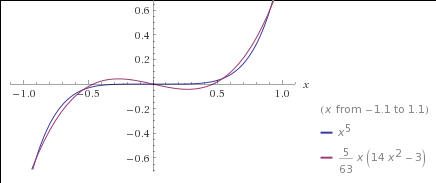
\includegraphics{InterpolationOfx^5.png}
\end{document}
